An availability issue may be caused by different types of anomalies.
For different anomaly types the quality metrics that are considered in service anomaly detection and the anomaly propagation directions that are considered in propagation chain analysis are different.
As shown in Table~\ref{table:issue}, the considered quality metrics for performance anomaly, reliability anomaly, and traffic anomaly are response time (RT), error count (EC), and queries per second (QPS), respectively.
The propagation directions for both performance anomaly and reliability anomaly are from downstream to upstream, while the propagation direction for traffic anomaly is from upstream to downstream.

\begin{table}
	\small
	\centering
	\caption{Metrics and Propagation Direction of Availability Issues}
	\vspace{-3mm}
	\label{table:issue}
	\begin{tabular}{|c|c|c|}
		\hline
		\textbf{Anomaly Type} & \textbf{Metric} & \textbf{Propagation Direction} \\
		\hline
		Performance Anomaly & RT & downstream $\rightarrow$ upstream \\
		\hline
		Reliability Anomaly & EC & downstream $\rightarrow$ upstream \\
		\hline
		Traffic Anomaly & QPS & upstream $\rightarrow$ downstream  \\
		\hline
	\end{tabular}
	\vspace{-3mm}
\end{table}

\begin{figure}[ht]
	\centering
	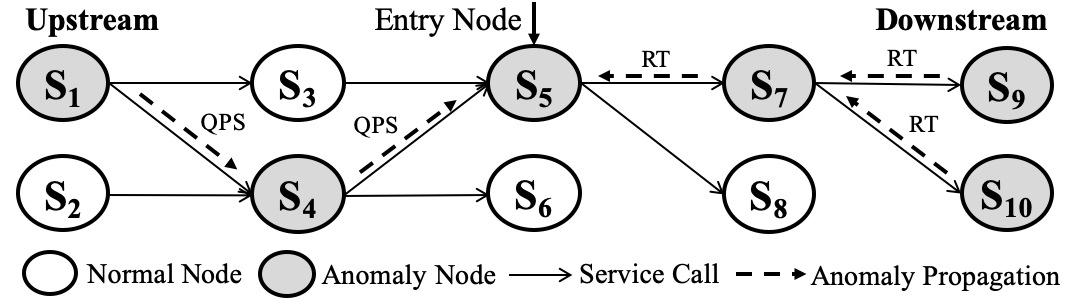
\includegraphics[width=0.5\textwidth]{images/propagation.png}
	\vspace{-8pt}
	\caption{Anomaly Propagation Chain Analysis Process}\label{fig:propagation}
	\vspace{-5pt}
\end{figure}

The process of the anomaly propagation chain analysis is shown in Figure~\ref{fig:propagation}.
It is performed on the service call graph in the following three steps.

\textbf{1) Entry Node Analysis}.
Treat the initial anomalous service in the service call graph as the entry node.
Conduct service anomaly detection for each of its neighboring nodes (i.e., those services that directly invoke or are directly invoked by the initial anomalous service) in terms of different anomaly types and the corresponding quality metrics.
For each detected neighboring anomalous node, if its upstream/downstream relationship with the entry node is consistent with the anomaly propagation direction of the detected anomaly type, start an anomaly propagation chain analysis from it and make the detected anomaly type as the anomaly type of the anomaly propagation chain.
For example, for the entry node $S_5$ in Figure~\ref{fig:propagation}, two neighboring anomalous nodes $S_4$ and $S_7$ are detected and their anomaly types are traffic anomaly and performance anomaly respectively.
As $S_4$ is an upstream node of $S_5$ and its relationship with $S_5$ is consistent with the anomaly propagation direction of traffic anomaly (from upstream to downstream), a traffic anomaly propagation chain analysis is started from $S_4$.
Similarly, a performance anomaly propagation chain analysis is started from $S_7$.

\textbf{2) Anomaly Propagation Chain Extension}.
For each anomaly propagation chain, iteratively extend it by backtracking along the anomaly propagation direction from the starting point (i.e., a detected neighboring anomalous node of the initial anomalous service).
In each iteration, conduct service anomaly detection for all the upstream/downstream nodes of the current node in terms of the anomaly type of the current anomaly propagation chain; for each detected upstream/downstream anomalous node, add it to the current anomaly propagation chain.
The extension of the anomaly propagation chain ends when no more nodes can be added to the chain.
For example, for the anomaly propagation chain of $S_4$ the extension ends with $S_1$, which is an upstream node of $S_4$ and conforms to the propagation direction of traffic anomaly to $S_4$.
Similarity, for the anomaly propagation chain of $S_7$ the extension ends with $S_9$ and $S_{10}$.

\textbf{3) Candidate Root Causes Output}.
When all the anomaly propagation chain analysis for the initial anomalous service ends, report all the services where the extension of an anomaly propagation chain ends as candidate root causes.
For example, the candidate root causes reported for the analysis process shown in Figure~\ref{fig:propagation} include $S_1$, $S_9$, and $S_{10}$.
